\section{Protokół Bluetooth Low Energy}
\label{bluetooth}

Poniższy podrozdział powstał na podstawie źródeł \cite{BLE} oraz \cite{inzynierka}.\\

Projekt protokołu BLE (\textit{ang. \textbf{B}luetooth \textbf{L}ow \textbf{E}nergy}) został zapoczątkowany przez firmę Wibree należącą do grupy Nokia. Celem nadrzędnym, który przyświecał jego autorom nie było utworzenie kolejnego protokołu, którego zastosowanie byłoby przesadnie szerokie. Zamiast tego, zdecydowali się oni na zaprojektowanie standardu radiowego, umożliwiającego najniższe możliwe zużycie energii, a przy tym nieskomplikowanego, przez co możliwe byłoby zastosowanie go w systemach o niskich kosztach budowy. Innymi słowy są to założenia idealne dla rynku smartfonów oraz IoT (\textit{ang. \textbf{I}nternet \textbf{o}f \textbf{T}hings}), gdzie urządzenia zasilane są z niewielkich baterii (często CR2032).

W trakcie prac, projekt został przejęty przez grupę Bluetooth SIG (\textit{ang. \textbf{B}luetooth \textbf{S}pecial \textbf{I}nterests \textbf{G}roup}), zrzeszającą dziesiątki firm i organizacji z wielu dziedzin przemysłu, zainteresowanych wykorzystywaniem i rozwojem protokołu Bluetooth. W roku 2010, Bluetooth Low Energy, znany również jako Bluetooth Smart został włączony do standardu Bluetooth 4.0 obok klasycznego protokołu Bluetooth Classic. Nie należy jednakże mylić tych dwóch protokołów komunikacyjnych, ponieważ poza warstwą fizyczną (interfejs radiowy o częstotliwości 2,4 GHz w pasmie ISM) znacznie różnią się w swych założeniach. Bluetooth Classic jest bowiem typowym protokołem umożliwiającym szybką, lecz energochłonną komunikację. W grudniu 2013 roku wprowadzono pierwszą dużą poprawkę do protokołu (Bluetooth 4.1), a rok później dalsze modyfikacje w postaci standardu Bluetooth 4.2. 

Bluetooth Low Energy, ze względu na swoje założenie o energoszczędności posiada pewne ograniczenia. Pierwszym z nich jest przepustowość danych. Górna granica prędkości transmisji wynosi 1 Mb/s, jednakże jest to wartość jedynie teoretyczna. W praktyce jest ona obwarowana wieloma ograniczeniami sprzętowymi producentów układów. W standardzie określono, że pojedynczy pakiet danych może zawierać maksymalnie 20 bajtów. Ograniczenie sprzętowe wynika tu z częstotliwości wysyłania pakietów. Dla  mikrokontrolera Nordic Semiconductor z rodziny nRF51, wynosi ona do 6 pakietów na każdy interwał połączenia. Jest to konfigurowalny parametr, określający odcinek czasu w obrębie którego jeśli nie dojdzie do transmisji pakietu, połączenie zostanie uznane za zerwane. Interwał połączenia może wynosić od 7,5 ms do 4 s. Przy założeniu najmniejszej wartości tego parametru otrzymujemy przepustowość:

\begin{equation}
	\text{Przepustowość} = 6 \text{pakietów/interwał} \cdot \frac{1000ms}{7,5ms} \cdot 20 \text{bajtów} = 15960 \text{bajtów/s} \approx 128 Kb/s
\end{equation}

Jak widać, jest to wartość znacznie odbiegająca od 1 Mb/s, jednakże w porównaniu do zysku na zużyciu energii jest to i tak bardzo dobry wynik. 

Kolejne ograniczenie to zasięg komunikacji. Oficjalnie, Bluetooth Low Energy posiada zasięg rzędu 50 m. Jest to jednak wartość trudna do uzyskania, silnie zależna od otoczenia (między urządzeniami nie może być przeszkód), mocy transmisji (rekonfigurowalna, im mniejsza tym mniejszy zasięg) oraz liczby innych urządzeń znajdujących się w pobliżu. Duża liczba nadajników BLE wpływa na zajętość kanałów komunikacyjnych i dodatkowo zmniejsza przepustowość łącza. Pasmo częstotliwości (od 2,402 GHz do 2,480 GHz), wykorzystywanej przez protokół podzielone jest na 40 kanałów. Przedstawiono to na rysunku \ref{fig:image_ble_channels}.

\begin{figure}[H]
	\centering
	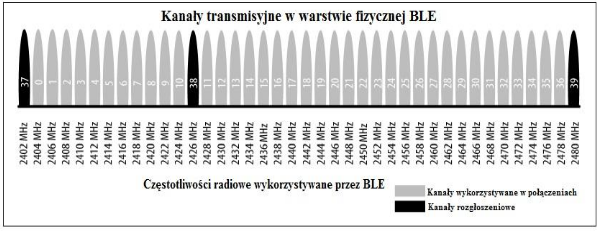
\includegraphics[width=17cm]{img/theory/BLE/ble_channels.png}
	\caption{Struktura pasma 2,4 ISM wykorzystywanego przez Bluetooth Low Energy.\\Źródło: \cite{inzynierka}.}
	\label{fig:image_ble_channels}
\end{figure}

Protokół Bluetooth Low Energy oferuje dwie możliwości wysyłania danych. Pierwszym z nich jest bezpołączeniowe rozgłaszanie (\textit{ang. Advertising}). Wówczas, każde z urządzeń wysyła cyklicznie  w eter pakiet danych o pojemności do 31 bajtów. Interwał między pakietami może wynosić od 20 ms do 10,24 s. Jest to jednak komunikacja jednokierunkowa. Wysłane w ten sposób dane może odebrać każde urządzenie będące w zasięgu.

\begin{figure}[H]
	\centering
	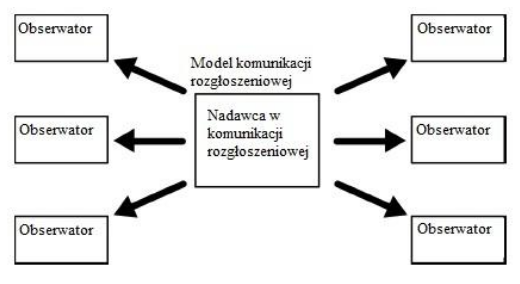
\includegraphics[width=12cm]{img/theory/BLE/ble_advertising.png}
	\caption{Model komunikacji rozgłoszeniowej. Źródło: \cite{inzynierka}.}
	\label{fig:image_ble_advertising}
\end{figure}

Drugą metodą jest wysyłanie danych będąc w połączeniu. Wówczas komunikacja może być dwustronna. W tym przypadku, BLE definiuje dwa możliwe typy urządzeń. Jedno z nich, które inicjuje połączenie określane jest jako \textit{Central}, natomiast urządzenie akceptujące połączenie - \textit{Peripheral}. Nie występuje przy tym ograniczenie, że urządzenie może mieć tylko jedną rolę. Może ono będąc w połączeniu urządzeniem typu \textit{Peripheral} zainicjować samodzielnie połączenie z innym odbiornikiem, a więc stać się dla tego połączenia \textit{Central'em}. Ważne jest, że dla danego połączenia, realizowanego typu punkt - punkt, urządzenie posiada tylko jedną rolę. 

Standard Bluetooth Low Energy definiuje logiczny podział struktur danych. Główną jednostką są tak zwane serwisy. Są to zgrupowania pewnych funkcjonalności, zwanych charakterystykami. Charakterystyki stanowią podstawowe jednostki komunikacji. Mogą one zawierać tzw. deskryptory, które są krótkimi, zrozumiałymi dla ludzi informacjami, jak na przykład nazwa charakterystyki. Można to porównać do definicji klasy (serwis), zawierającej definicje metod (charakterystyki). Struktura ta zarządzana jest przez serwer GATT (\textit{ang. \textbf{G}eneric \textbf{Att}ribute Server}). Przedstawiono ją na rysunku \ref{fig:image_ble_services}. 

\begin{figure}[H]
	\centering
	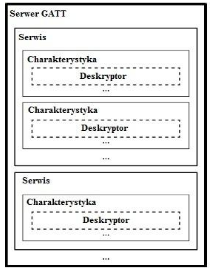
\includegraphics[width=5cm]{img/theory/BLE/ble_services.png}
	\caption{Model struktury danych serwera GATT. Źródło: \cite{inzynierka}.}
	\label{fig:image_ble_services}
\end{figure}

Dla charakterystyk zostały zdefiniowane 4 metody komunikacji. Pierwsza z nich - \textit{Write}, polega na wysłaniu danych z urządzenia typu \textit{Central} do \textit{Peripheral}. Druga - \textit{Read}, umożliwia inicjatorowi połączenia odczytanie danych z urządzenia podległego. Pozostałe 2 metody - \textit{Notify} oraz \textit{Indicate} polegają na wysłaniu danych z urządzenia typu \textit{Peripheral} do urządzenia typu \textit{Central} lub odwrotnie, bez żadnego żądania transmisji ze strony odbiorcy. Różnica polega na tym, że \textit{Indicate} wymaga od odbiornika wysłania potwierdzenia odbioru, a \textit{Notify} nie.

